% Document basé sur :
% BlaBLaTeX – Free Lab / Project Report Template
% https://www.blablatex.com
% Free to download, adapt and redistribute.

\documentclass[10pt,a4paper]{report}

%------------------------------------------------
% Encoding & language
%------------------------------------------------
\usepackage[T1]{fontenc}
\usepackage[utf8]{inputenc}
\usepackage[english]{babel}

%------------------------------------------------
% Page layout
%------------------------------------------------
\usepackage{geometry}
\geometry{
  a4paper,
  margin=2.4cm
}

\usepackage{setspace}
\onehalfspacing

\usepackage[parfill]{parskip}

\usepackage{lipsum}
\usepackage{titlesec}
\titlespacing{\chapter}
{0pt}{0.5ex plus 1ex minus .2ex}{1.3ex plus .2ex}

\usepackage{enumitem}
\setlist{noitemsep}

% Fix fancyhdr warning about headheight
\setlength{\headheight}{15pt}

%------------------------------------------------
% Fonts and math (Palatino-like)
%------------------------------------------------
\usepackage{amsmath,amssymb,amsthm}
\usepackage{newpxtext,newpxmath}

%------------------------------------------------
% Colors, graphics, plots, tables
%------------------------------------------------
\usepackage{xcolor}
\usepackage{graphicx}
\usepackage{booktabs}
\usepackage{siunitx}

\usepackage{tikz}
\usetikzlibrary{arrows.meta,positioning}

\usepackage{pgfplots}
\pgfplotsset{compat=1.18}

\sisetup{
  detect-all,
  table-number-alignment = center
}

% Color palette
\definecolor{DarkBlue}{HTML}{1f4e79}   % deep blue 1D1D5E
\definecolor{MediumBlue}{HTML}{2f75b5} % medium blue 1A1AD5
\definecolor{LightBlue}{HTML}{E3F2FD}   % very light blue
\definecolor{DarkText}{HTML}{102027}   % dark text gray
\definecolor{LightText}{HTML}{5a5a5a}   % light text gray 808080

\color{DarkText}

%------------------------------------------------
% Hyperlinks & clever references
%------------------------------------------------
\usepackage[hidelinks]{hyperref}
\usepackage{cleveref}

% Tell cleveref how to name listings
\crefname{lstlisting}{listing}{listings}
\Crefname{lstlisting}{Listing}{Listings}

%------------------------------------------------
% Theorem-like environments
%------------------------------------------------
\newtheorem{theorem}{Theorem}[chapter]
\newtheorem{proposition}[theorem]{Proposition}
\newtheorem{lemma}[theorem]{Lemma}
\newtheorem{corollary}[theorem]{Corollary}

\theoremstyle{definition}
\newtheorem{definition}[theorem]{Definition}
\newtheorem{example}[theorem]{Example}

\theoremstyle{remark}
\newtheorem{remark}[theorem]{Remark}

%------------------------------------------------
% Code listings
%------------------------------------------------
\usepackage{listings}
\lstdefinestyle{blablaListing}{
  basicstyle=\ttfamily\small,
  numbers=left,
  numberstyle=\tiny,
  stepnumber=1,
  numbersep=8pt,
  backgroundcolor=\color{LightBlue!30},
  frame=single,
  rulecolor=\color{LightBlue!80},
  keywordstyle=\color{DarkBlue}\bfseries,
  commentstyle=\color{gray},
  stringstyle=\color{MediumBlue},
  tabsize=2,
  breaklines=true,
  breakatwhitespace=true,
  showstringspaces=false
}
\lstset{style=blablaListing}

%------------------------------------------------
% Simple keywords environment
%------------------------------------------------
\newenvironment{keywords}{
  \par\vspace{0.5\baselineskip}\noindent
  \textbf{Keywords:}
}{\par\vspace{0.5\baselineskip}}

%------------------------------------------------
% Metadata commands
%------------------------------------------------
% Métadonnées
\newcommand{\reporttype}{Rapport technique}
\newcommand{\reporttitle}{Analyse et prédiction de la variabilité de la production solaire à partir de données ouvertes de la région PACA}
\newcommand{\reportsubtitle}{Prédiction à court terme de la variabilité de la production solaire photovoltaïque}
\newcommand{\reportpromo}{Promotion Data Scientist (AUG-2025)}
\newcommand{\reportauthorMI}{Moustafa IBRAHIM}
\newcommand{\reportauthorCC}{Christophe CRESTEY}
\newcommand{\reportauthorMB}{Mathilde BLANCHARD}
\newcommand{\reportlogo}{img/logo_liora.jpg}

% Footer signature (used in every page footer)
\newcommand{\footerrapport}{\small Analyse et prédiction de la variabilité photovoltaïque — Region PACA}

%------------------------------------------------
% Section titles
%------------------------------------------------
\usepackage{titlesec}

\titleformat{\chapter}[hang]
  {\normalfont\Huge\bfseries\color{DarkBlue}}
  {\thechapter.}{0.8em}{}

\titleformat{\section}[hang]
  {\normalfont\Large\bfseries\color{MediumBlue}}
  {\thesection}{0.8em}{}

\titleformat{\subsection}[hang]
  {\normalfont\large\bfseries\color{LightBlue}}
  {\thesubsection}{0.8em}{}

\titleformat{\subsubsection}[hang]
  {\normalfont\bfseries\color{DarkText}}
  {\thesubsubsection}{0.8em}{}

\titleformat{\caption}[hang]
  {\normalfont\itshape\color{LightText}}
  {\thecaption}{0.8em}{}

%------------------------------------------------
% Headers and footers
%------------------------------------------------
\usepackage{fancyhdr}
\pagestyle{fancy}
\fancyhf{} % clear

\fancyhead[L]{\nouppercase{\leftmark}}
\fancyhead[R]{\nouppercase{\rightmark}}
\fancyfoot[L]{\footerrapport}
\fancyfoot[R]{\thepage}

\fancypagestyle{plain}{
  \fancyhf{}
  \fancyfoot[L]{\footerrapport}
  \fancyfoot[R]{\thepage}
}

%------------------------------------------------
% Document
%------------------------------------------------
\begin{document}
\selectlanguage{french}

%---------------- Title page ----------------


\begin{titlepage}
    \centering

    % Logo
    \vspace*{0.5cm}
    \includegraphics[height=5cm]{\reportlogo}\par

    \vspace{3cm}

    % Title
    {\Large\bfseries\color{LightText}\reporttype\par}
    \vspace{0.4cm}
    {\LARGE\bfseries\color{DarkBlue}\reporttitle\par}
    \vspace{0.4cm}
    {\large\color{LightText}\reportsubtitle\par}

    \vspace{3cm}
    {\large\bfseries\color{LightText}\reportpromo\par}
    \vspace{0.6cm}
    {\color{LightText}\reportauthorMI\par}
    \vspace{0.1cm}
    {\color{LightText}\reportauthorCC\par}
    \vspace{0.1cm}
    {\color{LightText}\reportauthorMB\par}


\end{titlepage}

\tableofcontents

\chapter{Introduction}

La transition énergétique engagée en France et en Europe s’accompagne d’une montée en puissance
rapide des énergies renouvelables intermittentes, en particulier de la production photovoltaïque.
Longtemps marginale dans le mix électrique, cette filière occupe désormais une place croissante et sa
trajectoire de développement reste fortement orientée à la hausse dans les prochaines années :

\begin{figure}[htbp]
    \centering
    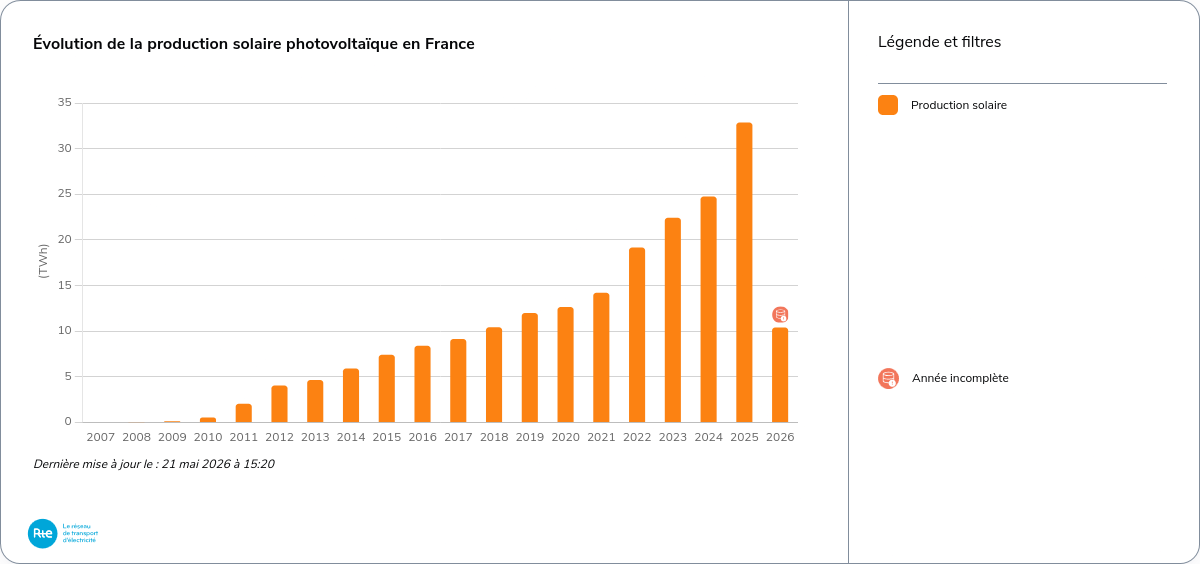
\includegraphics[width=0.7\textwidth]{img/evol_prod_fr.png}
    \caption{Évolution de la production solaire photovoltaïque en France.}
    \label{fig:evolFR}
\end{figure}

Cette figure illustre la croissance soutenue de la production photovoltaïque en France au cours des
dernières années. Cette augmentation rapide contribue à renforcer le rôle du solaire dans le mix
électrique, tout en accentuant les enjeux liés à la variabilité de la production et à son intégration dans le
système électrique. Source : RTE éCO2mix.

Cette évolution constitue un levier majeur de décarbonation du système énergétique, mais introduit
également une dépendance accrue aux conditions météorologiques, qui influencent directement la
disponibilité de la ressource solaire et donc la production effective d’électricité.

Cette transformation impacte particulièrement les réseaux de distribution, qui concentrent une part
importante des installations photovoltaïques décentralisées. Historiquement conçus pour des flux
essentiellement descendants, depuis des moyens de production centralisés vers les consommateurs,
ces réseaux doivent désormais gérer des injections locales variables, parfois importantes et difficilement
pilotables. Pour les gestionnaires de réseaux de distribution, cette évolution introduit de nouvelles
contraintes opérationnelles : risques de surtension, congestions temporaires, sollicitations accrues des
mécanismes de flexibilité, ou encore limitations ponctuelles de production (écrêtement). L’augmentation
continue de la puissance photovoltaïque installée accroît mécaniquement l’exposition à ces situations,
avec pour conséquence potentielle une part croissante d’énergie renouvelable produite mais non
valorisée faute de capacité d’absorption ou d’anticipation suffisante.

Si la prévision de production photovoltaïque fait déjà l’objet de nombreux travaux, notamment à horizon
day-ahead ou intra-journalier, ces approches visent principalement à estimer des niveaux moyens de
production. Or, pour certaines problématiques opérationnelles, les fluctuations rapides de production à
court terme, provoquées par les dynamiques nuageuses, les conditions atmosphériques ou les
variations rapides d’irradiance, constituent un enjeu complémentaire important. Dans ce contexte, le
projet s’est orienté vers une démarche visant à mieux comprendre les mécanismes physiques qui
gouvernent la variabilité photovoltaïque, à structurer un jeu de données enrichi combinant production
observée et variables exogènes explicatives, puis à explorer des approches de modélisation prédictive
adaptées à cette problématique. La richesse et la diversité des facteurs environnementaux susceptibles
d’influencer la production photovoltaïque rendent cette problématique particulièrement adaptée aux
approches de machine learning, capables d’exploiter simultanément de multiples variables explicatives,
de capturer des relations non linéaires complexes et d’aider à identifier les facteurs les plus
déterminants dans la dynamique observée. Cette orientation répondait également à une motivation
pédagogique forte de l’équipe projet, consistant à articuler compréhension physique des phénomènes
énergétiques et mise en œuvre de méthodes avancées de data science.

\section{Objectifs}

Réalisé dans le cadre du cursus \textbf{Data Scientist}, ce projet avait pour objectif de mettre en œuvre, sur une
problématique réelle liée à la transition énergétique, les principales compétences acquises au cours de
la formation : collecte et préparation de données, analyse exploratoire, feature engineering, modélisation
prédictive, évaluation de modèles et interprétation des résultats.

Le cas d’étude retenu portait sur la variabilité de court terme de la production photovoltaïque,
problématique particulièrement intéressante d’un point de vue data science en raison de la multiplicité
des facteurs explicatifs potentiels, de leur forte composante exogène et de la complexité des relations
non linéaires entre environnement physique et production observée.

L’ambition du projet était d’évaluer dans quelle mesure des approches de machine learning pouvaient
contribuer à mieux comprendre et modéliser cette dynamique, en exploitant simultanément un ensemble
riche de variables explicatives issues de sources hétérogènes (production observée, météorologie,
paramètres atmosphériques et données astronomiques).

Plus concrètement, les objectifs poursuivis étaient les suivants :

\begin{itemize}
\item ​Construire un pipeline de collecte et de préparation de données multi-sources cohérent et exploitable
pour un cas d’usage de modélisation ;

\item Explorer les mécanismes physiques influençant la production photovoltaïque et identifier les
variables explicatives pertinentes ;

\item Concevoir des variables dérivées (feature engineering) adaptées à la modélisation de la variabilité de
court terme ;

\item Formuler le problème sous l’angle d’une tâche de machine learning supervisé appliquée aux séries
temporelles ;

\item Expérimenter et comparer différentes approches de modélisation prédictive ;

\item Analyser les performances obtenues ainsi que la contribution relative des différentes variables
explicatives.
\end{itemize}

\clearpage

\section{Equipe}

L’équipe projet réunissait des profils complémentaires, combinant expertise métier, compétences
quantitatives et intérêt pour les approches datascience appliquées à des problématiques complexes.

\textbf{Moustafa Ibrahim} apportait une sensibilité forte aux aspects quantitatifs, mathématiques et à la
modélisation. Son approche a été particulièrement utile pour la formalisation du problème, l’analyse des
dynamiques temporelles et l’évaluation des approches prédictives testées dans le cadre du projet.

\textbf{Christophe Crestey} apportait une expertise métier liée aux systèmes électriques et aux problématiques
opérationnelles des réseaux de distribution, acquise au travers d’une expérience professionnelle dans le
secteur de l’énergie. Cette connaissance a contribué au cadrage du sujet, ainsi qu’à l’interprétation
métier des résultats obtenus. Le projet constituait également pour lui une opportunité d’approfondir
l’usage des techniques de machine learning appliquées au domaine de la data.

\textbf{Mathilde Blanchard} disposait d’un profil scientifique orienté vers l’analyse de données et les approches
d’intelligence artificielle. Son expertise a contribué à la structuration méthodologique du projet, à la
rigueur des analyses et à l’exploration des approches de modélisation, avec une appétence particulière
pour les mécanismes d’apprentissage automatique et leur mise en œuvre technique.

Dans l’ensemble, si l’expertise métier énergétique était plus marquée chez certains membres de
l’équipe, le projet s’inscrivait précisément dans une logique d’apprentissage, permettant de croiser
compréhension physique des phénomènes énergétiques et montée en compétence collective sur les
méthodes de data science.

\section{Interactions avec des experts métier}

Le projet n’a pas donné lieu à un dispositif formel d’entretiens structurés avec des experts externes
dédiés à la problématique. En revanche, le cadrage du sujet s’est appuyé sur une connaissance métier
préexistante des problématiques de réseaux électriques de distribution, notamment liées à l’intégration
croissante des productions renouvelables décentralisées.

L’expérience professionnelle de certains membres de l’équipe dans le secteur de l’énergie a permis
d’ancrer le projet dans des problématiques opérationnelles concrètes, telles que la gestion des
contraintes réseau, l’impact des fluctuations de production photovoltaïque sur l’exploitation, ou encore
les enjeux d’anticipation liés à l’intermittence des énergies renouvelables.

Au-delà de cette expertise embarquée, des échanges informels avec l’environnement professionnel ont
contribué à conforter la pertinence du sujet, notamment sur l’intérêt croissant porté aux problématiques
de prévision, de flexibilité et d’intégration des ENR dans les infrastructures électriques.

\clearpage

\section{Projets similaires, environnement métier}

Des problématiques proches existent déjà dans l’écosystème énergétique, notamment autour de la
prévision de production des énergies renouvelables, en particulier à des horizons day-ahead ou
intra-journaliers. Ces approches visent principalement à anticiper les niveaux de production agrégés
nécessaires à l’équilibrage du système électrique, à l’optimisation des mécanismes de marché ou à
l’exploitation opérationnelle des infrastructures électriques.

Le projet a également bénéficié d’une exploration approfondie de l’écosystème \textbf{open data énergétique},
qui constitue aujourd’hui une source particulièrement riche d’inspiration méthodologique et de données.
Les plateformes ouvertes telles que \textbf{RTE éCO2mix}, l’\textbf{Agence ODRE} (Open Data Réseaux Énergies),
\textbf{ENTSO-E}, ou encore différentes sources météorologiques ouvertes, illustrent la dynamique croissante
de mise à disposition de données énergétiques et environnementales exploitables dans des approches
de data science. Cette ouverture a fortement contribué au cadrage du projet, tant dans le choix des
variables étudiées que dans la structuration du pipeline de collecte et d’enrichissement des données.

Dans l’environnement professionnel de certains membres de l’équipe, les enjeux liés à l’intégration des
productions renouvelables distribuées, à l’anticipation des contraintes réseau et à l’exploitation de
données énergétiques sont des sujets bien identifiés. Toutefois, les approches observées sont
généralement orientées vers des usages opérationnels ciblés de prévision ou de supervision, plutôt que
vers une exploration explicite de la variabilité de court terme et de ses facteurs explicatifs physiques.

Le projet s’inscrit ainsi davantage comme une \textbf{démarche exploratoire de data science appliquée},
inspirée par les problématiques réelles du secteur énergétique et rendue possible par la richesse
croissante de l’open data, plutôt que comme la reproduction directe d’un dispositif existant.


\chapter{Cadrage géographique}

Le cadrage géographique du projet a constitué une étape méthodologique importante, directement liée à l’hétérogénéité spatiale des données disponibles. Si les données environnementales, météorologiques et astronomiques peuvent être obtenues à des résolutions spatiales fines, les données ouvertes de production photovoltaïque utilisées comme variable cible ne sont, pour leur part, disponibles publiquement qu’à une maille régionale agrégée via la plateforme \textbf{RTE éCO2mix} pour la filière photovoltaïque.

Cette asymétrie imposait de définir une stratégie permettant de rapprocher des variables explicatives locales d’une cible observée à une échelle plus large. Afin d’éviter une représentation trop simplificatrice de la région étudiée, un travail exploratoire de \textbf{clustering géographique} a été mené en amont.

L’approche retenue s’est appuyée sur la répartition géographique du parc de production photovoltaïque régional afin d’identifier plusieurs zones représentatives du territoire. L’objectif était de capturer la diversité des conditions environnementales susceptibles d’influencer la production observée, tout en restant cohérent avec le niveau d’agrégation de la cible. Cette démarche a conduit à la sélection de \textbf{cinq points géographiques représentatifs}, servant de points d’échantillonnage pour la collecte des variables météorologiques, atmosphériques et astronomiques.

Le choix de la région \textbf{Provence-Alpes-Côte d’Azur (PACA)} s’est imposé naturellement comme zone d’étude. La région combine en effet un fort niveau de pénétration photovoltaïque, une ressource solaire importante et une variabilité météorologique suffisamment marquée pour rendre le problème de modélisation particulièrement intéressant. Ce territoire offre ainsi un compromis favorable entre disponibilité des données, cohérence physique et intérêt opérationnel pour l’étude de la variabilité photovoltaïque.


\begin{figure}[htbp]
    \centering
    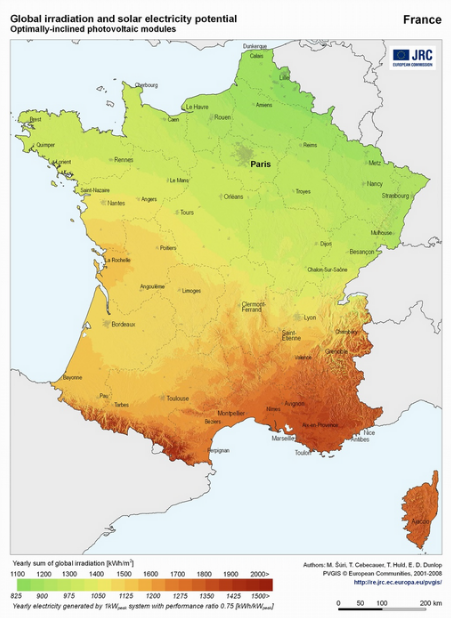
\includegraphics[height=7cm]{img/irradianceFR.png}
    \caption{Irradiance solaire annuelle moyenne en France.}
    \label{fig:irradianceFR}
\end{figure}

Cette carte représente la répartition spatiale de l’irradiance solaire annuelle moyenne sur le territoire français. Elle met en évidence un gradient Nord–Sud marqué, avec des niveaux d’irradiance plus élevés dans le sud du pays, notamment en région Provence-Alpes-Côte d’Azur. Cette distribution contribue à expliquer les disparités régionales observées en matière de production photovoltaïque.
Source : Commission européenne – PVGIS (JRC).


\chapter{Collecte de données}

Cette section décrit la collecte de données ouvertes permettant de calculer la variabilité du Taux de CHarge de la production solaire (TCH solaire) ainsi que de l’expliquer, de manière à permettre par la suite une modélisation robuste et basée sur des observations physiques pertinentes. On vise ainsi une prédiction de la variabilité du TCH à 30 minutes dans le futur, pour permettre aux opérateurs du réseau de prendre d’éventuelles mesures préventives sur le réseau électrique en cas de de forte variabilité.

\section{Données de production}

Des données de production d’énergie sur le territoire Français sont mises à disposition par RTE. Il est possible de télécharger ces données pour la région PACA sur le site éCO2mix (licence Etalab) : elles sont disponibles pour les années 2013 à 2025, à raison d’un jeu de données par année.

La première exploration de ces données montrent que la {\bfseries variabilité du TCH n’est pas disponible en l’état dans ces données} : il est donc nécessaire de la calculer, par exemple de la manière suivante (le détail de ce choix sera donné dans les sections suivantes) :

\begin{equation}
\left| V(t + \Delta t) \right| = \left| \frac{P(t+\Delta t) - P(t)}{P_{capacite}} \right| = \left| TCH(t + \Delta t) - TCH(t)\right| = \left| \Delta TCH(t + \Delta t) \right|
\end{equation}

Avec :
\begin{itemize}
\item $V$ : la valeur absolue de la variabilité du taux de charge de la production solaire (variable cible pour cette étude) ;
\item $P$ : la production d’énergie solaire (disponible pour toutes les années sous le nom Solaire’) ;
\item $P_{capacite}$ : la capacité du parc de production installé (varie au fil du temps, non disponible dans le jeu de données éCO2mix et complexe à reconstruire) ;
\item $TCH$ : le taux de charge de la production solaire (disponible pour les années 2020 à 2025)
\end{itemize}

L'objectif du projet sera donc de résoudre un problème de régression supervisée.

La variable idéale pour ce calcul est le TCH solaire, mais cette variable n’est disponible qu’à partir de l’année 2020. Entre 2020 et 2025, 106 704 observations sont disponibles dans éCO2mix, ce qui reste raisonnable pour cette étude : on décide donc de se limiter aux années 2020 à 2025.

Or les années 2020 à 2025 ne présentent {\bfseries pas toutes le même nombre de variables} : on commence par rechercher les variables communes puis on ne conserve dans ces variables communes que {\bfseries celles concernant la production d’énergie solaire}, ainsi que la consommation. Cette dernière variable pourrait en effet présenter un intérêt pour la modélisation car en cas de forte production mais de faible demande, les opérateurs du réseau peuvent être amenés à limiter la production d’énergie photovoltaïque, voire à la couper. Idéalement, le modèle final pourrait capter ce type de situation pour limiter la gêne occasionnée sur le réseau.

A cette étape, on conserve 6 variables : \textit{date}, \textit{heures}, \textit{consommation}, \textit{solaire}, \textit{tco\_solaire}, \textit{tch\_solaire} (le détail des variables sera donné dans la section Analyse exploratoire~\ref{subsec:var_dispo}).

Ces données ne contiennent aucun élément permettant d’expliquer la production d’énergie solaire : on sait que de nouvelles données explicatives devront être agrégées à ces premières variables collectées.

Or les variables idéales pour agréger de nouvelles données sont la date et l’heure des observations. On s’interroge alors sur le fuseau horaire utilisé par RTE : s’agit-il d’un fuseau UTC ou du fuseau horaire de France métropolitaine ? Les données explicatives fournies par RTE avec le jeu de données ne le précise pas.

On va donc observer comment varie la production d’énergie solaire entre deux dates où l’on sait qu’un changement d’heure à eu lieu en France métropolitaine. \textbf{Observe-t-on un décalage horaire dans la production} entre le jour avant et le jour suivant le changement d'heure ?

\begin{itemize}
\item Si oui : le fuseau horaire est bien celui de France métropolitaine ;
\item Sinon : le fuseau horaire est peut être le fuseau UTC.
\end{itemize}

\begin{figure}[htbp]
    \centering
    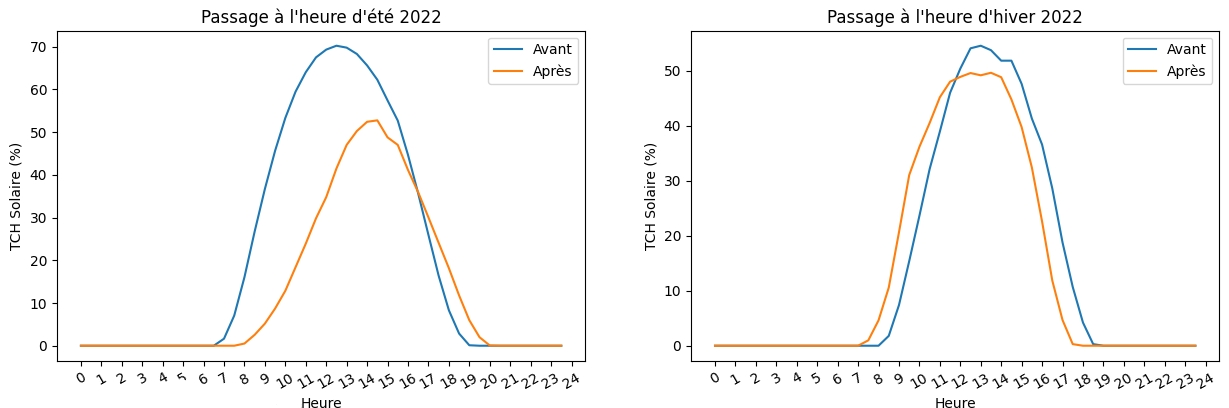
\includegraphics[width=0.8\textwidth]{img/heures_ete_hiver.jpg}
    \caption{Changements d'heure en 2022.}
    \label{fig:changement_heure}
\end{figure}

On observe bien un décalage horaire : la production est décalée une heure plus tard lors du passage à l’heure d’été et une heure plus tôt lors du passage à l’heure d’hiver.

La date et l’heure de France métropolitaine sont converties en une seule variable \textit{datetime\_utc}, de manière à pouvoir agréger de nouvelles données facilement par la suite (toutes les données suivantes seront collectées sur la base d’une heure UTC).

Pour clore cette première partie de la collecte de données, on calcule notre variable cible (valeur absolue de la variabilité du tch solaire à l’instant t + 30 minutes) : on dispose à ce stade de 106 704 observations pour 6 variables (\textit{datetime\_utc}, \textit{consommation}, \textit{solaire}, \textit{tco\_solaire}, \textit{tch\_solaire}, \textit{target}).

\begin{figure}[htbp]
    \centering
    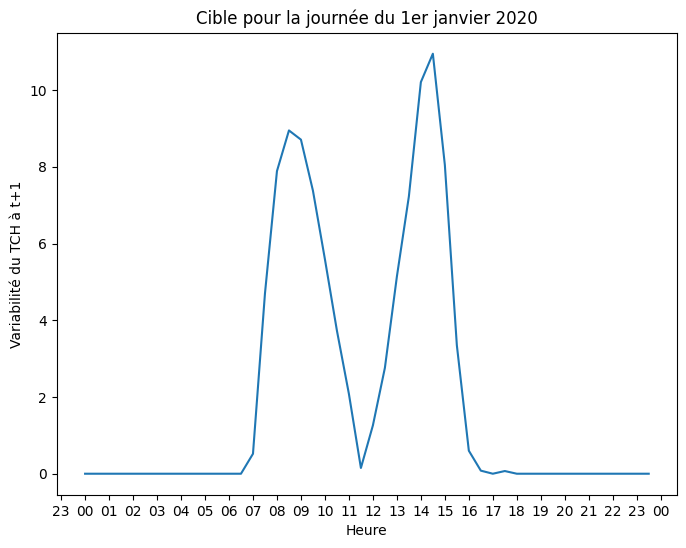
\includegraphics[height=5cm]{img/cible.png}
    \caption{Valeur absolue de la variabilité du Taux de CHarge de la production solaire (TCH).}
    \label{fig:cible}
\end{figure}

\textbf{Plus de détails} sur les opérations réalisées pour la collecte des données de production sont disponibles dans notebooks/02\_Collecte/02\_collecte\_01\_production.ipynb.

\section{Données astronomiques}

Les données de \textbf{production d'énergie solaire} sont collectées et la variable cible construite, mais les variables collectées ne permettent à priori pas d'expliquer la variable cible.

\begin{itemize}
\item Elles ne contiennent pas de données sur la \textbf{position du soleil} par rapport aux panneaux solaires ;
\item Ni de données météorologiques ;
\item Ni de données atmosphériques.
\end{itemize}

Pour déterminer quelles données pourraient permettre d'expliquer notre variable cible et pourraient être utiles à notre modélisation, on part des connaissances usuelles de l'homme du métier (voir les articles retenus dans les Annexes).

Parmi ces connaissances, on a constaté que la position du soleil par rapport à l'emplacement des panneaux solaires était importante et que cette position était déterminée par l'\textbf{azimut} et l'\textbf{angle solaire}.

On a vu que la région PACA était vaste et on a déterminé \textbf{cinq lieux significatifs} pour la production d'énergie solaire : on calcule l'azimut et l'angle solaire pour chacun d'eux, à l’aide de la librairie Python \textbf{PySolar}, librement mise à disposition par des passionnés d’astronomie, pour chaque date présente dans le jeu de données précédemment collecté.

\textbf{Plus de détails} sur les opérations réalisées pour la collecte des données astronomiques sont disponibles dans notebooks/02\_Collecte/02\_collecte\_02\_astronomie.ipynb.

\section{Données atmosphériques}

Pour l'homme du métier, d'autres données que celles concernant la position du soleil pourraient permettre d'expliquer notre variable cible et être utiles à notre modélisation. On s’intéresse dans cette section aux \textit{rayonnements solaires effectivements reçus} au niveau des panneaux solaires et donc à des données concernant l'\textbf{atmosphère}.

Ces données sont par exemple disponibles dans un jeu de données \textbf{CAMS solar radiation time-serie} mis gracieusement à disposition par Copernicus (\href{https://www.copernicus.eu/fr}{programme d’observation de la Terre de l’Union européenne}), sous licence CC BY 4.0.

Pour chacun des points d'intérêts identifiés pour la production d'énergie solaire, on collecte 4 variables concernant l’irradiance reçue au niveau des panneaux solaire (\textit{GHI}, \textit{BHI}, \textit{DHI} et \textit{BNI}) ainsi que leur 4 équivalents au sommet de l’atmosphère (\textit{valeur théorique maximale} obtenue par temps clair).

Ces variables sont collectées via une API dédiée entre la première et la dernière date de notre jeu de données, avec une \textbf{résolution temporelle de 15 minutes}. Comme les variables que nous sommes en train de collecter sont \textbf{cumulatives}, on les sommes deux à deux pour obtenir des données pour 30 minutes. On ne conserve ensuite que les observations dont la date est présente dans le jeu de données de production.

\textbf{Plus de détails} sur les opérations réalisées pour la collecte des données atmosphériques sont disponibles dans notebooks/02\_Collecte/02\_collecte\_03\_atmosphere.ipynb.

\section{Données météorologiques}

Pour terminer la collecte de données et compléter les variables explicatives, on cherche maintenant à récupérer des \textbf{informations météorologiques} complémentaires, telles que :

\begin{itemize}
\item La \textit{température} au sol (influe sur la performance des panneaux solaires) ;
\item La \textit{vitesse du vent} au sol (influe sur la performance des panneaux solaires) ;
\item L'\textit{humidité} (influe sur la performance des panneaux solaires) ;
\item La \textit{nébulosité} (influe sur la lumière reçue par les panneaux solaires).
\end{itemize}

On peut trouver ces données dans un dataset mis à disposition par la NASA via une API : \href{https://power.larc.nasa.gov/}{POWER Hourly API}, sous licence Creative Commons BY 4.0.

Cette base de données a une résolution temporelle d'une heure : comme les données précédentes ont une résolution de 30 minutes et qu’on souhaite garder cette précision pour notre variable cible, on interpole les données météorologiques.

Enfin, l’instrument de mesure de la nébulosité utilisé ici est arrivé en fin de vie le 30 décembre 2025 : les observations suivantes sont supprimées.

\textbf{Plus de détails} sur les opérations réalisées pour la collecte des données météorologiques sont disponibles dans notebooks/02\_Collecte/02\_collecte\_04\_meteorologie.ipynb.

\section{Bilan de la collecte}

Quatre jeux de données ont été collectés concernant la production d’énergie solaire, des données astronomiques, atmosphériques et météorologiques. Ces quatre jeux sont fusionnés en un seul jeu de données par un merge sur la variable \textit{datetime\_utc} commune à tous.



\chapter{Analyse exploratoire}

Les données brutes étant collectées, l’objectif est désormais de les analyser pour les comprendre et préparer le feature engineering avant de rechercher un modèle.

Dans cette section, nous allons :

\begin{itemize}
\item Faire le bilan des observations et des variables disponibles ;
\item Vérifier leur type ;
\item Vérifier si des valeurs sont manquantes ou aberrantes ;
\item Etudier leur relations potentielles.
\end{itemize}

\section{Variables disponibles}
\label{subsec:var_dispo}

Le jeu de données collecté comprend 86 variables pour 105 170 observations à une résolution temporelle de 30 minutes entre le 31 décembre 2019 (1er janvier 2020 heure française) et le 30 décembre 2025 (date de fin de service du satellite ayant collecté les données de nébulosité).

Aucune observation n’est manquante : le jeu de données comprend bien une et une seule observation toutes les 30 minutes du début à la fin de la collecte.

Par ailleurs, toutes les variables sont de type numérique (float64) à l’exception de la variable temporelle \textit{datetime\_utc} utilisée comme index (DatetimeIndex).

Enfin, il n’y a ni valeur manquante, ni doublons.

On dispose de 6 variables concernant l’ensemble de la région :

\begin{itemize}
\item \textbf{consommation} : consommation électrique totale du périmètre considéré sur l'intervalle de temps donné.
\item \textbf{datetime\_utc} : horodatage en temps universel coordonné (UTC) correspondant à l'instant d'agrégation des données (résolution 30 minutes).
\item \textbf{solaire} : production électrique issue des installations photovoltaïques sur le périmètre considéré.
\item \textbf{target} : variabilité absolue du taux de charge de la production solaire à t + 30 minutes (notre variable cible).
\item \textbf{tco\_solaire} : taux de couverture de la production solaire.
\item \textbf{tch\_solaire} : taux de charge de la production solaire.
\end{itemize}

Outre ces six variables à l’échelle régionale, on dispose de 16 variables pour les cinq points d'intérêts de la production photovoltaïque régionale (ce qui représente 16 x 5 = 80 colonnes) :

\begin{itemize}
\item \textbf{altitude} : altitude solaire (en degrés), représentant l'élévation du soleil au-dessus de l'horizon (valeurs négatives durant la nuit).
\item \textbf{azimuth} : azimut solaire (en degrés), indiquant la direction du soleil par rapport au nord (0–360° selon la convention).
\item \textbf{bhi} \textit{(Beam Horizontal Irradiance)} : composante directe du rayonnement solaire projetée sur le plan horizontal (Wh/m²).
\item \textbf{bni} \textit{(Beam Normal Irradiance)} : irradiance directe normale, reçue sur un plan perpendiculaire aux rayons solaires (Wh/m²).
\item \textbf{clear\_sky\_bhi} : composante directe horizontale en conditions de ciel clair (Wh/m²).
\item \textbf{clear\_sky\_bni} : irradiance directe normale en conditions de ciel clair (Wh/m²).
\item \textbf{clear\_sky\_dhi} : composante diffuse horizontale en conditions de ciel clair (Wh/m²).
\item \textbf{clear\_sky\_ghi} : irradiance globale horizontale en conditions de ciel clair, utilisée comme référence théorique sans nuages (Wh/m²).
\item \textbf{dhi} \textit{(Diffuse Horizontal Irradiance)} : composante diffuse du rayonnement solaire reçue sur un plan horizontal (Wh/m²).
\item \textbf{ghi} \textit{(Global Horizontal Irradiance)} : irradiance globale reçue sur un plan horizontal (composantes directe et diffuse) exprimée en Wh/m².
\item \textbf{humidite} : humidité de l'air (généralement humidité relative en %, ou humidité spécifique selon la source).
\item \textbf{nebulosite} \textit{(souvent cloud\_AMT)} : nébulosité ou fraction de couverture nuageuse (exprimée selon les produits en fraction, pourcentage ou indice adimensionnel).
\item \textbf{reliability} : fiabilité des données CAMS (\textit{bhi}, \textit{bni}, \textit{clear\_sky\_bhi}, \textit{clear\_sky\_bni}, \textit{clear\_sky\_dhi}, \textit{clear\_sky\_ghi}, \textit{dhi}, \textit{ghi}, \textit{toa}).
\item \textbf{temperature} \textit{(souvent T2M)} : température de l'air à 2 mètres du sol (en °C ou en K selon la source ; une vérification des unités est nécessaire).
\item \textbf{toa} \textit{(Top Of Atmosphere)} : rayonnement solaire incident au sommet de l'atmosphère (Wh/m²), utilisé pour le contrôle de cohérence et la normalisation des séries.
\item \textbf{vitesse\_vent} \textit{(souvent V2M)} : vitesse du vent mesurée à 2 mètres du sol (m/s).
\end{itemize}

\begin{figure}[htbp]
    \centering
    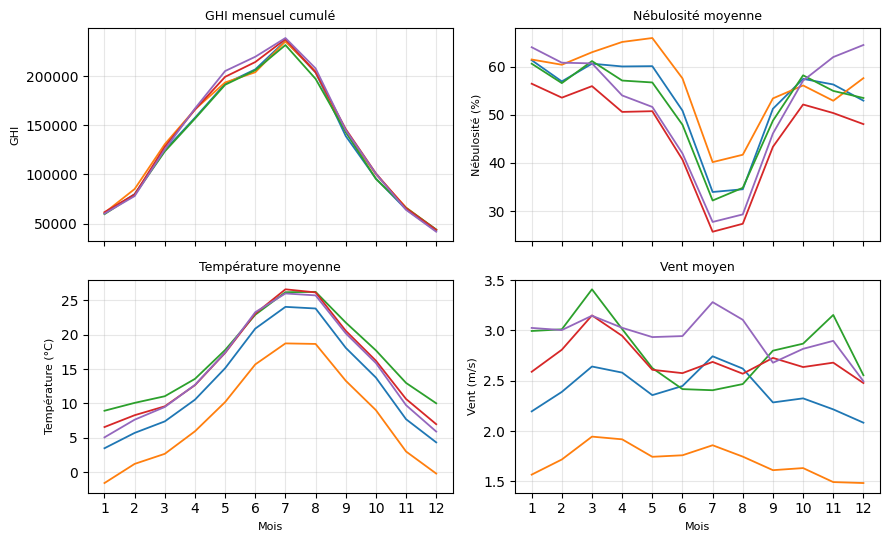
\includegraphics[width=0.9\textwidth]{img/ex_meteo.png}
    \caption{Comparaisons de variables prises aux cinq points significatifs.}
    \label{fig:comparaisons_5pts}
\end{figure}

On remarque toutefois qu’à quelques exceptions près (dhi, nébulosité et vitesse du vent), chacune de ces variables présente une forte colinéarité entre elles, ce que confirme une analyse du VIF (Variance Inflation Factor).

\textbf{Plus de détails} sur les tests statistiques sur les variables communales sont disponibles dans notebooks/03\_Analyse/03\_analyse\_01\_exploration\_preliminaire.ipynb.

Afin de faciliter l’analyse de ces variables communales, on décide de les remplacer par leur somme pondérée par la contribution des communes correspondantes à la production d’énergie solaire régionale.

Exemple pour la variable GHI :

\begin{equation}
GHI_{region} = \sum_{i=1}^{5}p_{i}.GHI_{i}
\end{equation}

Avec :

\begin{itemize}
\item $GHI_{region}$ la somme pondérée obtenue pour remplacer les cinq variables GHI communales ;
\item $i$ une commune parmis les cinq communes d’intérêt ;
\item $GHI_{i}$ la valeur de la variable GHI dans la commune i ;
\item $p_{i}$ le poid correspondant à la part de la contribution à la production photovoltaïque de la région par la commune i.
\end{itemize}

\section{Distribution des variables}

Afin d’explorer la distribution des variables météorologiques régionales construites par agrégation pondérée, une analyse exploratoire est réalisée à l’aide de boxplots.

Exemple pour les variables mesurées au niveau communale :

\begin{figure}[htbp]
    \centering
    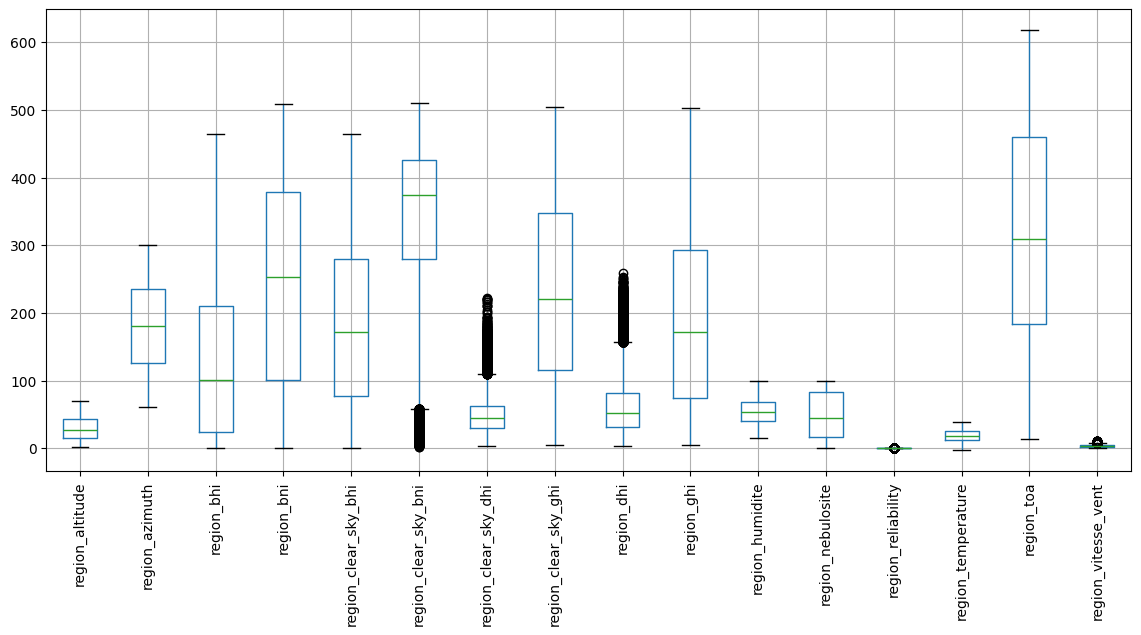
\includegraphics[width=0.9\textwidth]{img/distrib_5pts.png}
    \caption{Distributions des variables mesurées au niveau communal puis aggrégées.}
    \label{fig:distrib_5pts}
\end{figure}

Les distributions des variables sont diverses : les échelles de valeurs diffèrent parfois de deux ordres de grandeur. Une normalisation des données pourra être pertinente pour certains algorithmes de modélisation.

Les variables \textit{region\_clear\_sky\_bhi}, \textit{region\_clear\_sky\_dhi} et \textit{region\_dhi} présentent des valeurs extrêmes, mais celles-ci ne paraissent pas aberrantes.

Il en va de même pour les variables collectées directement au niveau régional.

L’étude de la variance des variables permet de constater que la variable \textit{reliability} (qui concerne la fiabilité des données atmosphériques) a une variance inférieure à 0.01, ce qui la rend peu exploitable en pratique : elle sera mise de côté lors de l’étape de feature engineering.

\section{Exploration de la variable cible}

Dans cette section, nous allons explorer la manière dont se comporte notre variable cible au cours d’une journée, d’une année et par rapport aux variables TCH solaire et GHI. D’autres études ont été menées dans le notebook correspondant (cité en fin de section).

On s’intéresse tout d’abord à l’évolution moyenne de la variable cible et de la production d’énergie solaire (tch solaire) au cours d’une journée, en excluant la nuit où le soleil est couché :

\begin{figure}[htbp]
    \centering
    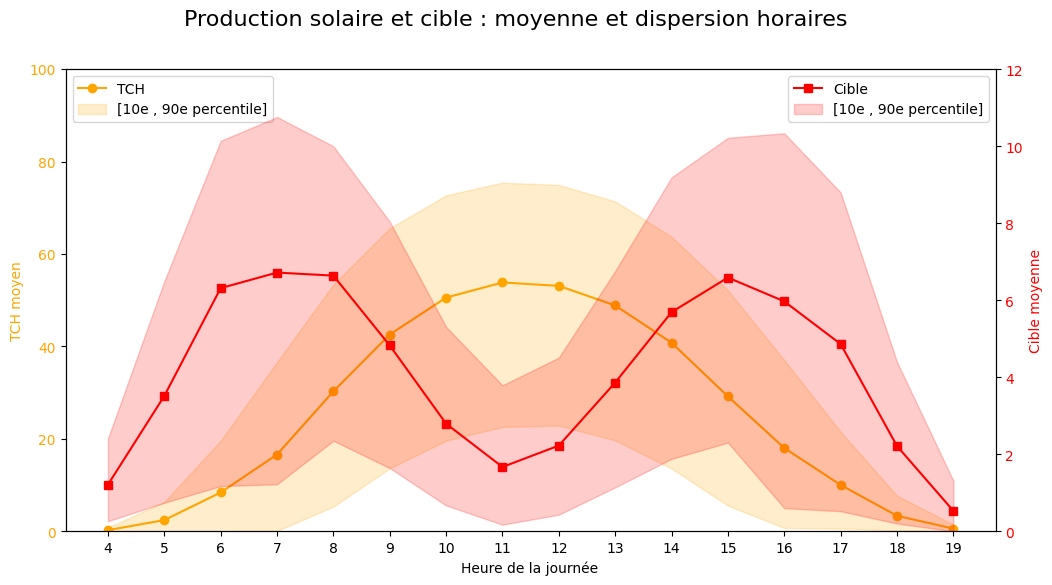
\includegraphics[width=0.9\textwidth]{img/cible_tch_jour.png}
    \caption{Comparaison du TCH et de sa variabilité au cours de la journée : moyenne et dispersion.}
    \label{fig:cible_tch_jour}
\end{figure}

\begin{itemize}
\item La production solaire est \textbf{faible et relativement instable en proportion} en début et fin de journée (variabilité élevée).
\item Elle est \textbf{maximale et la plus régulière autour de midi}, caractérisée par une \textbf{forte moyenne et une faible variabilité}.
\end{itemize}

Cette analyse permet d'identifier les \textbf{heures les plus stables} (milieu de journée) et celles où la \textbf{variabilité est la plus forte} (matin et après-midi).

\clearpage

Si on s’intéresse maintenant aux statistiques saisonnières, on constate :

\begin{figure}[htbp]
    \centering
    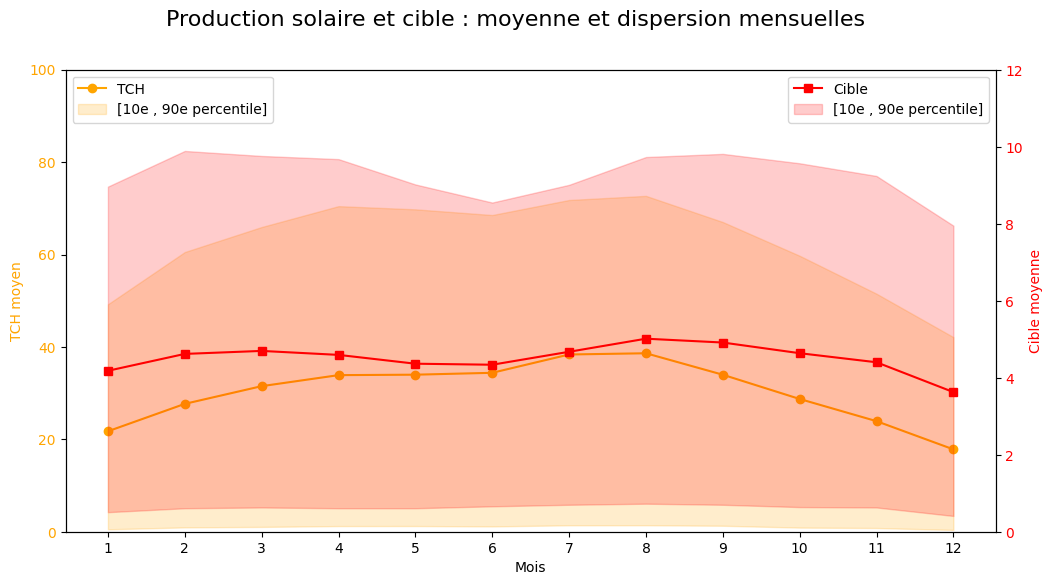
\includegraphics[width=0.7\textwidth]{img/cible_tch_mois.png}
    \caption{Comparaison du TCH et de sa variabilité au cours de l'année : moyenne et dispersion.}
    \label{fig:cible_tch_mois}
\end{figure}

\begin{itemize}
\item Que la \textit{cible} est plus \textbf{faible} et plus \textbf\textbf en \textbf{mai et juin} ainsi qu'en \textbf{décembre et en janvier} ;
\item Qu’en automne et en hiver, la production est \textbf{plus régulière relativement à son niveau moyen}.
\end{itemize}

Enfin on peut également analyser la variation de la variable cible et du tch solaire en fonction de la variable GHI qui témoigne de l’irradiance solaire reçue au niveau des panneaux solaires :

\begin{figure}[htbp]
    \centering
    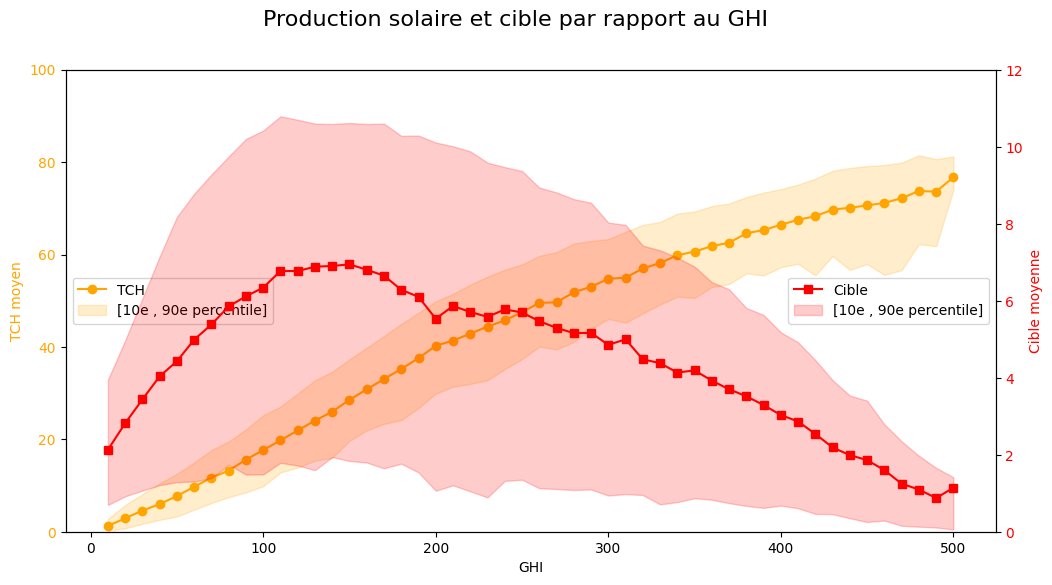
\includegraphics[width=0.7\textwidth]{img/cible_tch_ghi.png}
    \caption{TCH et variabilité du TCH en fonction du GHI : moyenne et dispersion.}
    \label{fig:cible_tch_ghi}
\end{figure}

\begin{itemize}
\item La moyenne de TCH augmente régulièrement avec le GHI, ce qui traduit une relation cohérente entre irradiance et production.
\item La variabilité de la production solaire est faible aux faibles GHI (peu de production au lever et coucher du jour), atteint un maximum vers GHI = 150, ce indique une variabilité relative importante pour une production moyenne faible. Au-delà de cette valeur du GHI, la variabilité de la production solaire diminue progressivement lorsque le GHI augmente : la production devient alors plus stable proportionnellement à sa moyenne.
\end{itemize}

\textbf{Plus de détails} sur les distributions des variables et leurs relation entre elles sont disponibles dans notebooks/03\_Analyse/03\_analyse\_02\_exploration\_detaillee.ipynb.


\chapter{Feature Engineering}

Cette partie décrit la transformation des données brutes en jeux de données exploitables par les modèles de Machine Learning. L'objectif n'est pas seulement d'ajouter un grand nombre de variables, mais de construire des variables cohérentes avec la physique du phénomène étudié et compatibles avec une prédiction en temps réel. Chaque variable explicative doit donc être disponible à l'instant de prédiction ou dans le passé. Cette règle est essentielle pour éviter toute fuite d'information depuis le futur.

La cible du projet est la variabilité future de la production photovoltaïque normalisée, mesurée à l'horizon de 30 minutes. En pratique, le modèle cherche à prédire l'amplitude de la variation future plutôt que son signe. La formulation retenue est :

\begin{equation}
target(t) = |TCH\_solaire(t + \Delta t) - TCH\_solaire(t)|
\end{equation}

Avec : $\Delta t = 30 minutes$

Cette définition permet de se concentrer sur les épisodes de stabilité ou d'instabilité de la production solaire. Une valeur élevée de la cible correspond à une variation importante de la production sur le prochain pas de temps, ce qui est particulièrement utile pour anticiper les rampes photovoltaïques.

\begin{figure}[htbp]
    \centering
    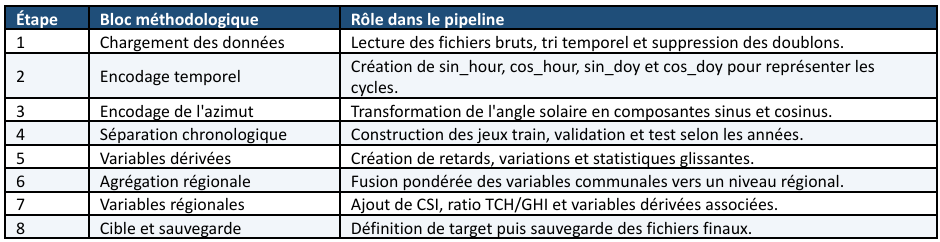
\includegraphics[width=0.9\textwidth]{img/pipe_fe.png}
    \caption{Chaîne générale du feature engineering.}
    \label{fig:pipe_fe}
\end{figure}

\section{Objectif et principe général}

Le feature engineering part du jeu de données principal couvrant plusieurs années d'observations. Les variables disponibles incluent notamment des informations de production, des variables radiatives, des variables météorologiques, des variables solaires géométriques et des observations associées à plusieurs points représentatifs de la région PACA. Le notebook identifie cinq points d'intérêt, repérés par les préfixes \textit{cru}, \textit{sel}, \textit{svt}, \textit{bra} et \textit{eyg}. Cette organisation permet d'automatiser les mêmes transformations sur chaque point.

Un principe directeur est conservé tout au long de la préparation : les transformations doivent reproduire les conditions d'une utilisation future du modèle. Ainsi, les variables retardées et les statistiques glissantes sont construites à partir du passé. Les variables qui utiliseraient directement la valeur future de la production ne sont pas intégrées comme variables explicatives.

\section{Encodages temporels et angulaires}

Les phénomènes photovoltaïques sont fortement cycliques. La production dépend de l'heure de la journée, de la position dans l'année et de la position apparente du soleil. Utiliser directement l'heure ou le jour de l'année comme des entiers créerait des discontinuités artificielles : par exemple, 23 h et 0 h sont proches dans la réalité, mais éloignés numériquement. Pour éviter ce problème, les variables cycliques sont encodées sous forme de sinus et de cosinus.

\begin{figure}[htbp]
    \centering
    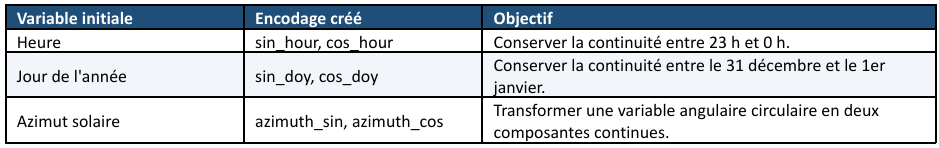
\includegraphics[width=0.9\textwidth]{img/tab2.png}
    \caption{Encodages cycliques utilisés pour les variables temporelles et angulaires.}
    \label{fig:tab2}
\end{figure}

\begin{figure}[htbp]
    \centering
    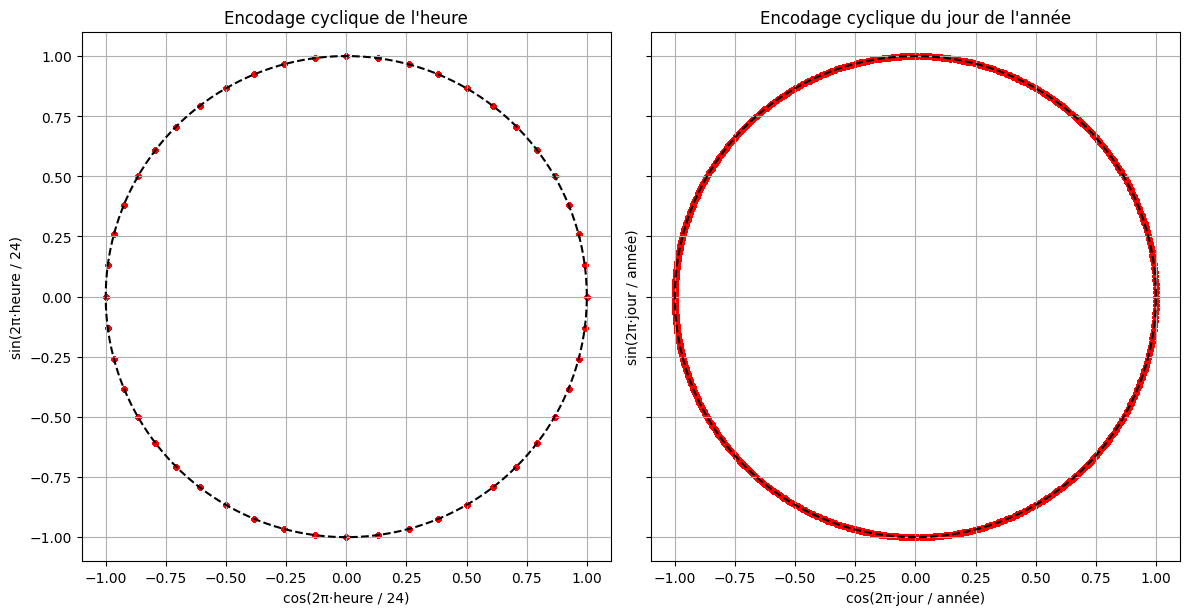
\includegraphics[width=0.9\textwidth]{img/cycle1.png}
    \caption{Vérification de l'encodage cyclique de l'heure et du jour de l'année.}
    \label{fig:cycle1}
\end{figure}

\begin{figure}[htbp]
    \centering
    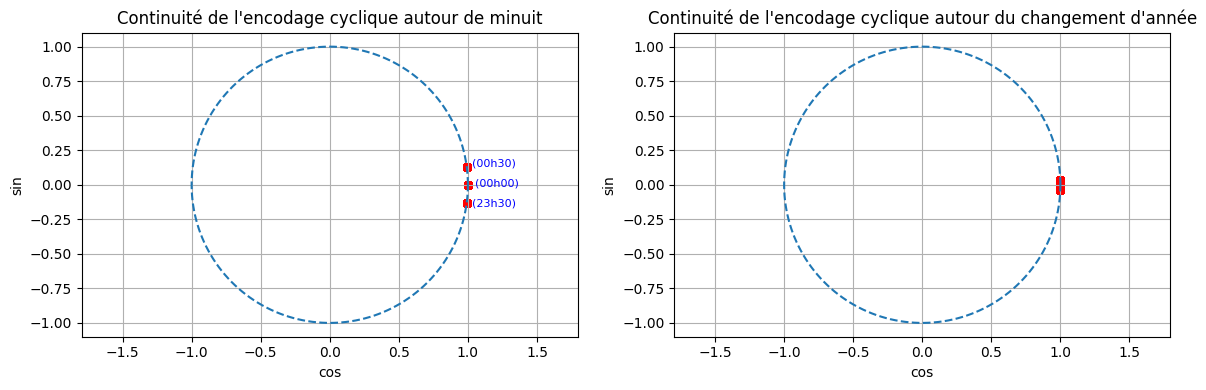
\includegraphics[width=0.9\textwidth]{img/cycle2.png}
    \caption{Continuité autour de minuit et du changement d'année.}
    \label{fig:cycle2}
\end{figure}


Les figures montrent que les points se placent sur un cercle unité. Cette représentation garantit que deux instants proches dans le cycle restent proches dans l'espace des variables, même lorsqu'ils se situent de part et d'autre d'une frontière numérique. Cet encodage est particulièrement important pour les modèles d'arbres et les modèles linéaires, car il évite d'introduire une rupture artificielle dans les données.

\section{Variables dérivées communales}

Après les encodages cycliques, le notebook ajoute des variables décrivant la dynamique récente des grandeurs physiques. La variabilité solaire à court terme est souvent liée à des changements rapides d'irradiance, à la nébulosité et à la variation récente de la production. Pour cette raison, plusieurs familles de variables sont enrichies par des retards, des variations instantanées et des statistiques glissantes.

\begin{figure}[htbp]
    \centering
    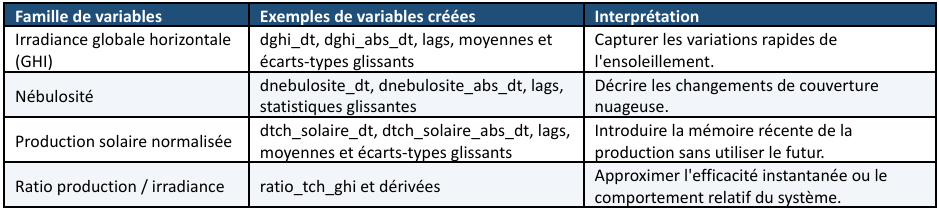
\includegraphics[width=0.9\textwidth]{img/tab3.png}
    \caption{Exemples de variables dérivées construites dans le notebook.}
    \label{fig:tab3}
\end{figure}

Les variables de retard permettent au modèle d'observer la mémoire courte du système. Les variations absolues mesurent l'intensité des changements récents, tandis que les statistiques glissantes sur deux heures résument l'état récent du ciel et de la production. Cette combinaison est pertinente pour un problème de variabilité : il ne suffit pas de connaître la valeur actuelle d'une variable, il faut aussi connaître la dynamique qui précède cette valeur.

Le notebook applique les mêmes transformations aux ensembles d'entraînement, de validation et de test. Ce choix assure que les trois jeux de données possèdent la même structure de colonnes. Il facilite également la reproductibilité du pipeline et limite le risque d'erreurs manuelles.

\section{Nettoyage, séparation temporelle et sauvegarde intermédiaire}

Les retards et les fenêtres glissantes introduisent naturellement des valeurs manquantes au début des séries temporelles. Ces lignes sont supprimées après la création des variables. Les colonnes sont ensuite triées afin de rendre les fichiers plus lisibles et de faciliter les vérifications.

\begin{figure}[htbp]
    \centering
    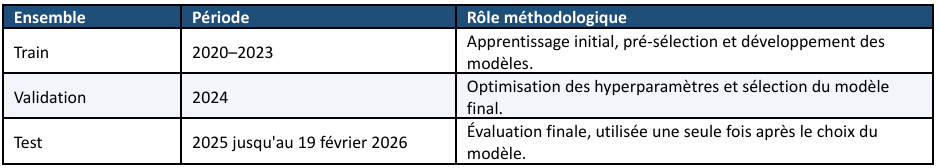
\includegraphics[width=0.9\textwidth]{img/tab4.png}
    \caption{Séparation chronologique des données pour éviter la fuite temporelle.}
    \label{fig:tab4}
\end{figure}


Le choix d'une séparation temporelle est fondamental. Un découpage aléatoire mélangerait des observations passées et futures, ce qui pourrait conduire à une évaluation trop optimiste. La validation sur 2024 et le test sur une période postérieure reproduisent une situation plus réaliste : entraîner le modèle sur le passé et vérifier sa capacité à généraliser dans le futur.

\clearpage

\section{Agrégation régionale et variables complémentaires}

Le notebook construit d'abord une version détaillée avec les variables de cinq points représentatifs. Cette représentation est riche, mais elle augmente fortement le nombre de colonnes. Pour la modélisation finale, une version régionale est ensuite créée. Les variables communales présentes pour les cinq points sont agrégées au niveau régional, puis les colonnes communales devenues inutiles sont supprimées.

Cette étape réduit la dimension du problème tout en conservant une information spatiale synthétique. Elle est cohérente avec l'objectif du projet, qui consiste à prédire la variabilité régionale de la production solaire plutôt que la dynamique d'une seule commune.

\begin{figure}[htbp]
    \centering
    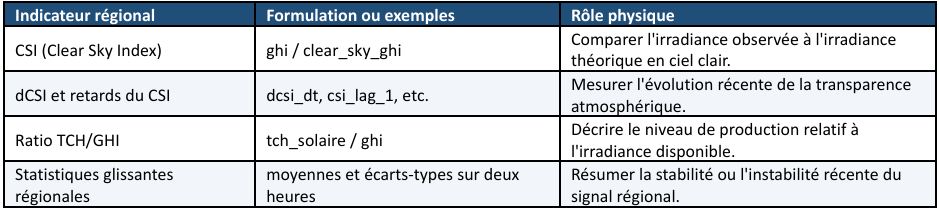
\includegraphics[width=0.9\textwidth]{img/tab5.png}
    \caption{Variables régionales complémentaires ajoutées après l'agrégation.}
    \label{fig:tab5}
\end{figure}

Le CSI est particulièrement utile : il donne une indication de l'écart entre les conditions réelles et les conditions de ciel clair. Des variations importantes de CSI peuvent correspondre à des passages nuageux ou à des transitions atmosphériques rapides, souvent associées à des variations de production. Le ratio TCH/GHI complète cette information en reliant directement la production solaire à l'irradiance disponible.

\section{Bilan du feature engineering}

Chaque ligne contient les informations disponibles au temps présent ou dans le passé, et la cible indique l'amplitude de la variation qui se produira au pas suivant.

À l'issue de cette étape, les fichiers régionaux finaux sont prêts pour le notebook de modélisation. Cette transition marque le passage d'une logique de préparation des données vers une logique d'évaluation et de sélection de modèles.


\chapter{Modélisation}

La modélisation commence à partir des fichiers régionaux produits par le feature engineering. L'objectif est d'entraîner plusieurs familles de modèles afin de prédire la variabilité future de la production solaire normalisée. La démarche est volontairement progressive : partir d'une baseline simple, tester des modèles linéaires interprétables, explorer des modèles plus complexes, puis sélectionner un modèle final selon des critères de performance et de généralisation.

\section{Organisation des ensembles et métriques}

Les jeux de données chargés dans le notebook contiennent les variables régionales finales et la cible \textit{target}. Après séparation entre variables explicatives et cible, les tailles utilisées pour la modélisation sont les suivantes :

\begin{figure}[htbp]
    \centering
    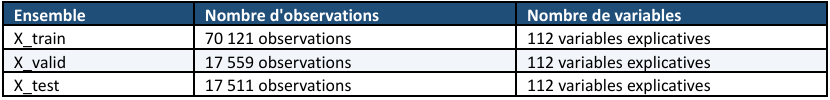
\includegraphics[width=0.8\textwidth]{img/tab_6_1.png}
    \caption{Dimensions des ensembles utilisés après séparation entre X et y.}
    \label{fig:tab_6_1}
\end{figure}

Comme les données sont temporelles, la validation croisée est également construite de manière chronologique. Chaque fold entraîne le modèle sur une période passée et le valide sur une période future. Cette stratégie permet d'évaluer la stabilité temporelle des modèles et d'éviter la fuite d'information.

\begin{figure}[htbp]
    \centering
    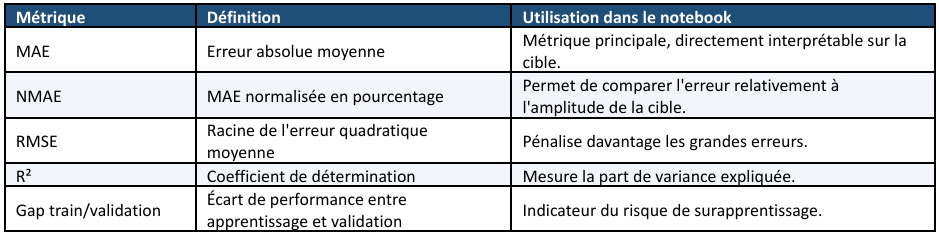
\includegraphics[width=0.9\textwidth]{img/tab_6_2.png}
    \caption{Métriques utilisées pour comparer les modèles.}
    \label{fig:tab_6_2}
\end{figure}

La MAE est privilégiée car elle mesure directement l'erreur moyenne sur l'amplitude de la variabilité prédite. Cependant, la sélection finale ne repose pas uniquement sur la MAE. Le RMSE et le gap entre entraînement et validation sont également considérés pour éviter de retenir un modèle trop optimiste ou trop instable.

\section{Baseline naïve et modèles linéaires}

La première étape consiste à établir un niveau minimal de performance. La baseline naïve prédit que la variabilité future sera proche de la dernière variation absolue observée de la production solaire normalisée, représentée par la variable \textit{dtch\_solaire\_abs\_dt}. Cette référence est importante : un modèle avancé doit faire mieux que cette règle simple pour être réellement utile.

\begin{figure}[htbp]
    \centering
    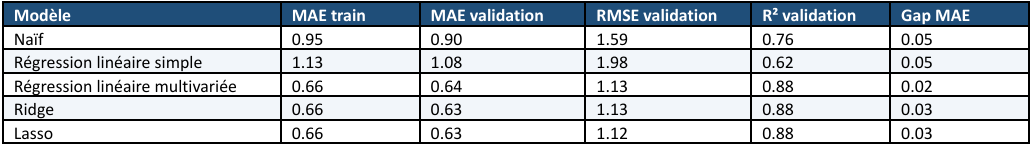
\includegraphics[width=0.9\textwidth]{img/tab_6_3.png}
    \caption{Performances des références naïves et linéaires sur validation.}
    \label{fig:tab_6_3}
\end{figure}

La régression linéaire simple basée uniquement sur la variation de GHI reste inférieure à la baseline naïve. Cela montre que la variabilité de la production ne peut pas être expliquée correctement par une seule variable radiative. Les modèles linéaires multivariés améliorent nettement les performances et atteignent un R² de validation proche de 0,88. Ils constituent donc une référence solide, mais ils restent moins performants que les modèles non linéaires optimisés.

\section{Sélection exploratoire et optimisation des modèles}

Après les modèles linéaires, on utilise le modèle LazyPredict pour obtenir une première comparaison rapide de plusieurs familles de modèles. Cette étape n'est pas utilisée comme évaluation finale, mais elle oriente le choix des modèles à optimiser plus finement. Les modèles d'arbres et de boosting apparaissent comme les plus prometteurs.

\begin{figure}[htbp]
    \centering
    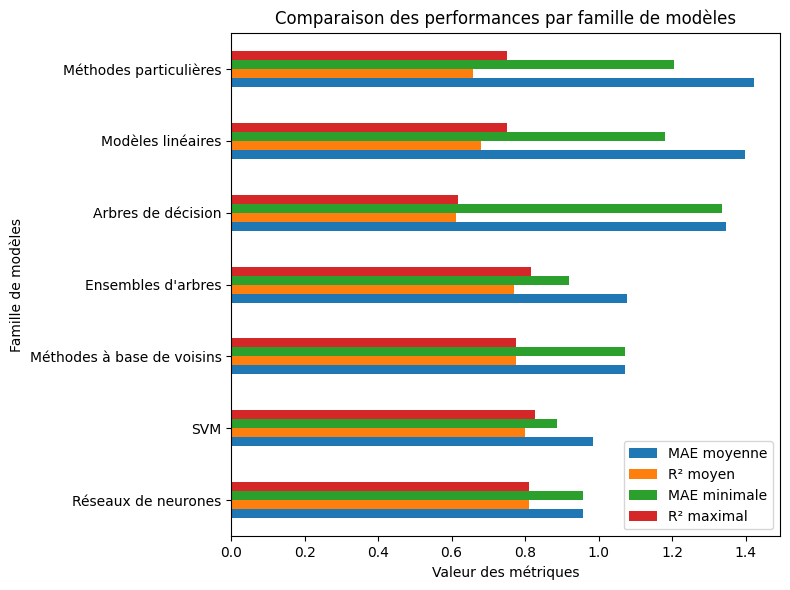
\includegraphics[width=0.8\textwidth]{img/metriques.png}
    \caption{Comparaison exploratoire des performances par famille de modèles.}
    \label{fig:metriques}
\end{figure}

Les modèles retenus pour l'optimisation détaillée comprennent LightGBM, XGBoost, ExtraTreesRegressor, RandomForestRegressor, HistGradientBoostingRegressor et un réseau de neurones MLP. Les hyperparamètres sont optimisés avec Optuna en utilisant les folds temporels définis manuellement. Cette méthode permet de tester de nombreuses combinaisons tout en respectant la structure chronologique des données.

\clearpage

\begin{figure}[htbp]
    \centering
    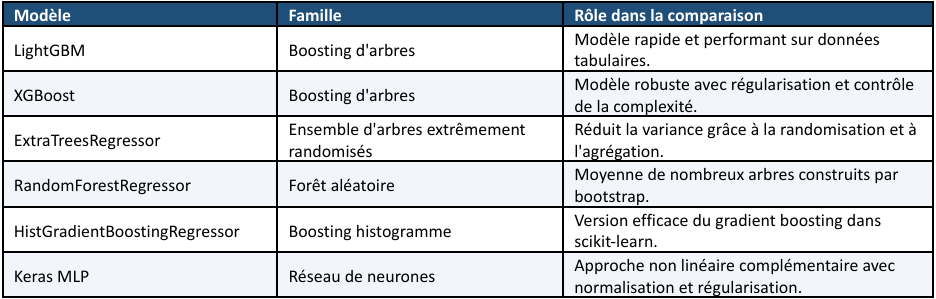
\includegraphics[width=0.9\textwidth]{img/tab_6_4.png}
    \caption{Familles de modèles optimisées dans le notebook.}
    \label{fig:tab_6_4}
\end{figure}

Les visualisations réel/prédit sur validation complètent les métriques numériques. Elles permettent de repérer si les modèles suivent correctement la tendance générale ou s'ils saturent pour les fortes variations. Ces figures montrent globalement une bonne concentration autour de la diagonale, mais aussi une dispersion plus importante pour les valeurs élevées de variabilité, ce qui est fréquent dans les problèmes de rampes solaires.

\begin{figure}[htbp]
    \centering
    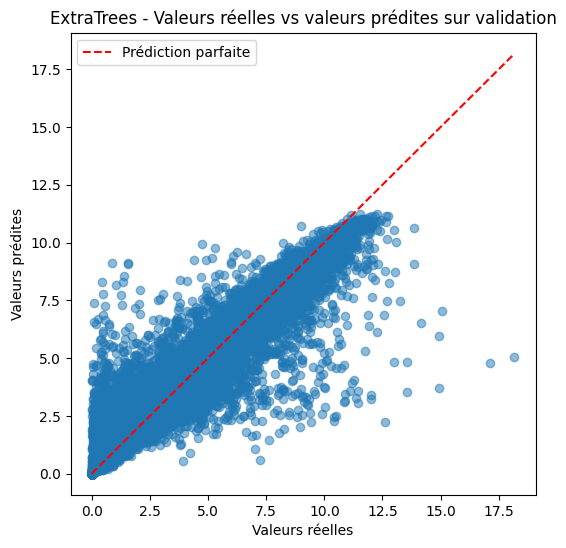
\includegraphics[width=0.5\textwidth]{img/extra_trees.png}
    \caption{ExtraTrees : valeurs réelles et prédites sur l'ensemble de validation.}
    \label{fig:extra_trees}
\end{figure}

\section{Choix du modèle final et évaluation sur test}

Après l'optimisation, les modèles sont comparés à partir d'un score combinant la MAE de validation, le RMSE de validation et le gap de MAE entre entraînement et validation. Ce score est donné par la formule :

\begin{equation}
score = MAE_{valid} + RMSE_{valid} + \frac{Gap_{MAE}}{MAE_{valid}}
\end{equation}

Cette stratégie évite de choisir uniquement le modèle avec la plus petite erreur moyenne si ce modèle présente un comportement moins stable.

\clearpage

\begin{figure}[htbp]
    \centering
    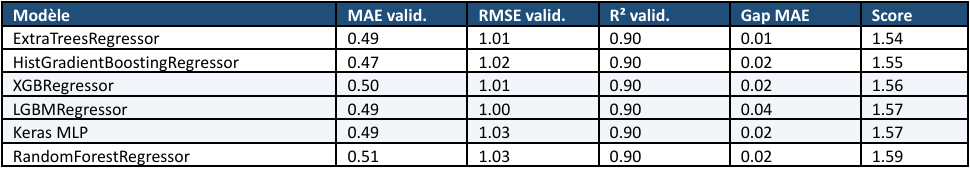
\includegraphics[width=0.9\textwidth]{img/tab_6_5.png}
    \caption{Classement des principaux modèles avant l'évaluation finale sur test.}
    \label{fig:tab_6_5}
\end{figure}

\begin{figure}[htbp]
    \centering
    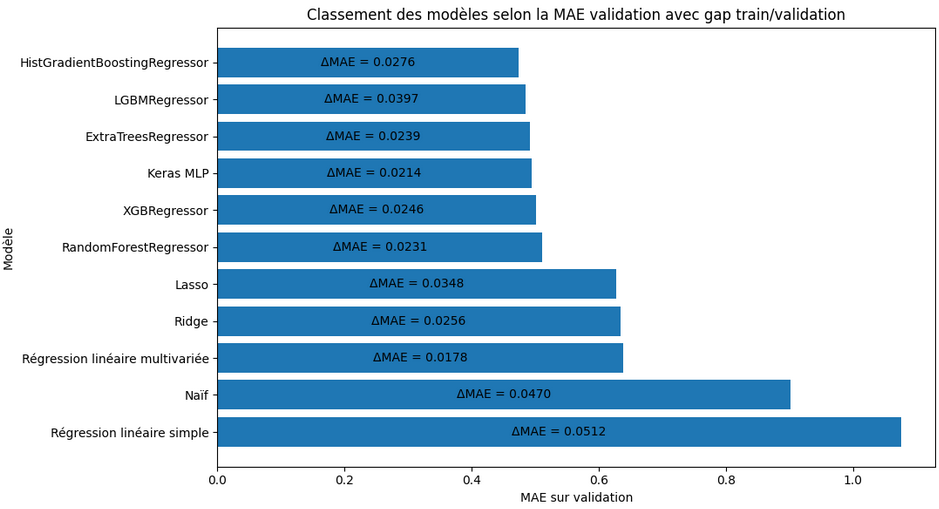
\includegraphics[width=0.9\textwidth]{img/classement.png}
    \caption{Classement des modèles selon le score de validation.}
    \label{fig:classement}
\end{figure}

Le modèle retenu est \textbf{ExtraTreesRegressor}. Il n'est pas seulement performant en validation : il présente aussi un écart train/validation faible et un bon compromis entre MAE, RMSE et R². Une fois ce choix effectué, le modèle est réentraîné sur l'ensemble de développement, c'est-à-dire la réunion de train et validation, puis évalué une seule fois sur le test.

\begin{figure}[htbp]
    \centering
    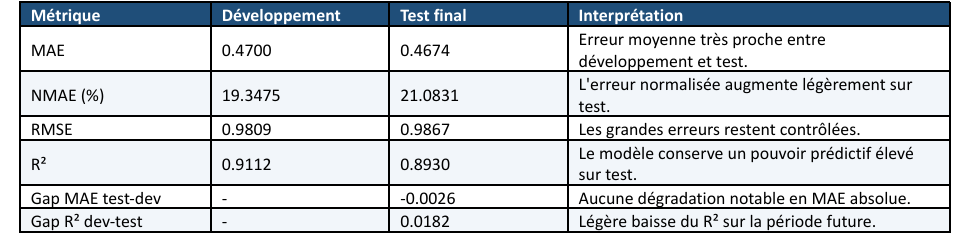
\includegraphics[width=0.9\textwidth]{img/tab_6_6.png}
    \caption{Évaluation finale du modèle ExtraTreesRegressor sur le jeu de test.}
    \label{fig:tab_6_6}
\end{figure}

\clearpage

\begin{figure}[htbp]
    \centering
    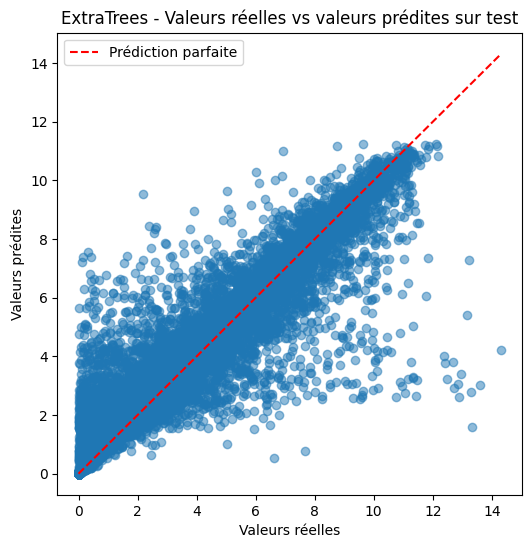
\includegraphics[width=0.5\textwidth]{img/pred_test.png}
    \caption{ExtraTrees : valeurs réelles et prédites sur l'ensemble de test.}
    \label{fig:pred_test}
\end{figure}

Les résultats finaux montrent que le modèle généralise correctement sur la période de test. La MAE est presque identique entre développement et test, tandis que le R² diminue légèrement. Cette baisse peut être liée à une modification de la distribution des données, à des conditions météorologiques différentes ou à une fréquence plus importante de cas extrêmes. Néanmoins, le R² test reste proche de 0,89, ce qui confirme la capacité du modèle à expliquer une part importante de la variabilité future.


\chapter{Interprétabilité du modèle final}

Après la sélection et l'évaluation du modèle final, l'analyse ne s'arrête pas aux métriques. Il est nécessaire de comprendre quelles variables influencent les prédictions et si ces variables ont une signification physique cohérente. Le modèle retenu étant un ensemble d'arbres, trois approches complémentaires sont utilisées : l'importance native des variables, les valeurs SHAP et la permutation importance.

\section{Importance native des variables}

L'importance native des variables mesure la contribution moyenne de chaque variable dans les divisions des arbres. Elle fournit une première lecture rapide du comportement du modèle. Cette méthode doit cependant être interprétée avec prudence, car elle peut être influencée par les corrélations entre variables.

\begin{figure}[htbp]
    \centering
    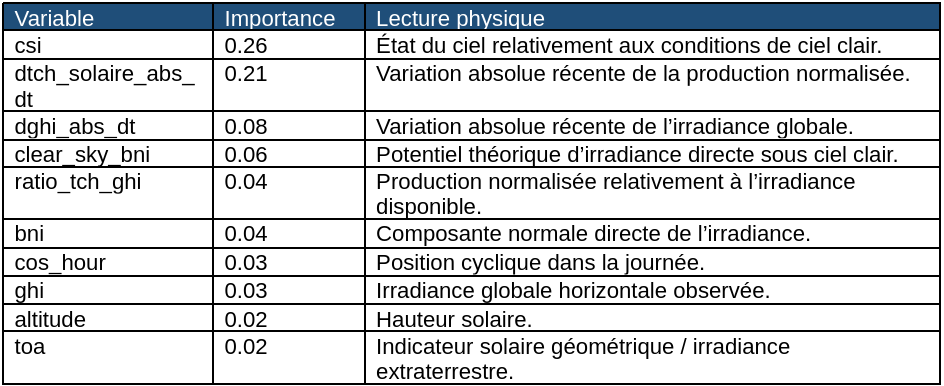
\includegraphics[width=0.7\textwidth]{img/tab_7_1.png}
    \caption{Dix premières variables selon l'importance native du modèle ExtraTrees.}
    \label{fig:tab_7_1}
\end{figure}

\begin{figure}[htbp]
    \centering
    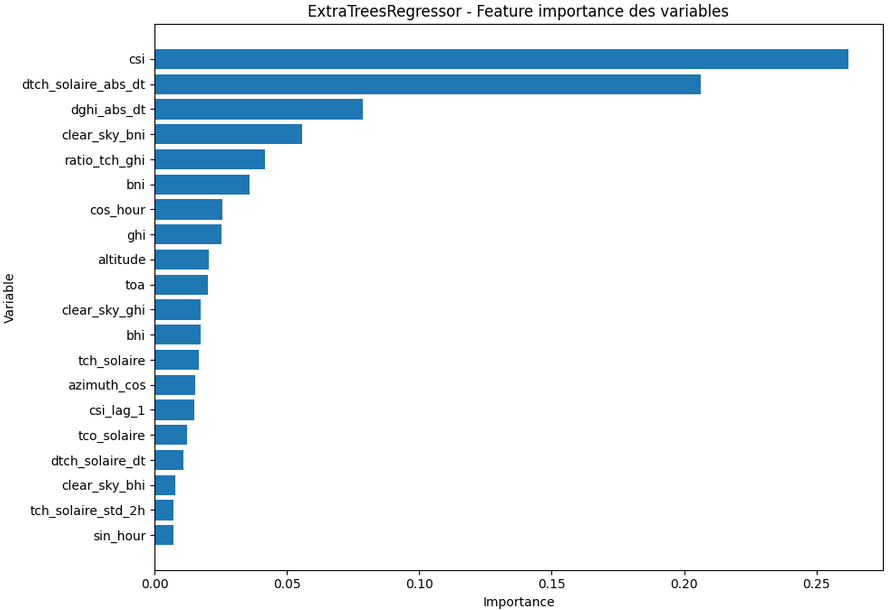
\includegraphics[width=0.7\textwidth]{img/var_nat_imp.png}
    \caption{Importance native des vingt premières variables du modèle ExtraTrees.}
    \label{fig:var_nat_imp}
\end{figure}

Les variables les plus importantes sont \textit{csi}, \textit{dtch\_solaire\_abs\_dt}, \textit{dghi\_abs\_dt} et \textit{clear\_sky\_bni}. Le modèle utilise donc principalement l'état du ciel par rapport au ciel clair, l'instabilité récente de la production, la variation récente de l'irradiance globale et le potentiel théorique d'irradiance directe par ciel clair.

Ce résultat est physiquement cohérent : la variabilité photovoltaïque à court terme dépend fortement de l'état atmosphérique, des changements récents d'irradiance et de la capacité du moment étudié à produire une variation visible de production.

\section{Analyse SHAP}

L'analyse SHAP apporte une interprétation plus détaillée que l'importance native. Elle estime, pour chaque observation, la contribution de chaque variable à la prédiction du modèle. Une valeur SHAP positive augmente la variabilité photovoltaïque prédite, tandis qu'une valeur SHAP négative la diminue.


\begin{figure}[htbp]
    \centering
    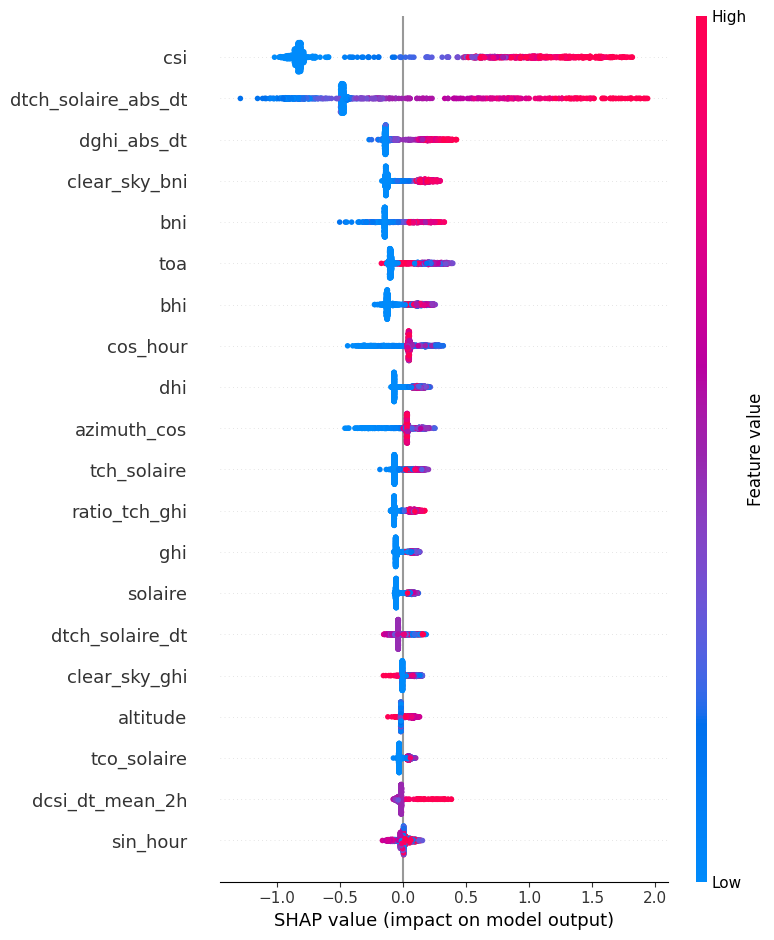
\includegraphics[height=0.5\textheight]{img/shap.png}
    \caption{Résumé SHAP : effet des variables sur les prédictions.}
    \label{fig:shap}
\end{figure}

Les résultats SHAP confirment que le modèle apprend principalement trois types d'information : l'état du ciel par rapport au ciel clair, l'instabilité récente de la production solaire normalisée et les variations récentes de l'irradiance. Les variables les plus influentes sont notamment \textit{csi}, \textit{dtch\_solaire\_abs\_dt}, \textit{clear\_sky\_bni} et \textit{dghi\_abs\_dt}.

Le \textit{csi} indique si le rayonnement observé est proche des conditions de ciel clair. Lorsqu'il est élevé, le potentiel de production est important et une perturbation atmosphérique peut entraîner une variation plus visible de la production. De même, \textit{clear\_sky\_bni} apporte un contexte physique sur le potentiel de rayonnement direct disponible selon la position du soleil, ce qui aide le modèle à identifier les périodes où une forte variation est possible.

La variable \textit{dtch\_solaire\_abs\_dt} mesure l'instabilité récente de la production. Lorsqu'elle est élevée, elle pousse généralement la prédiction vers une variabilité future plus importante, ce qui est cohérent avec l'idée qu'un système déjà instable peut rester instable à court terme. Enfin, \textit{dghi\_abs\_dt} et les autres variables radiatives, comme \textit{GHI}, \textit{DHI} ou \textit{BNI}, permettent d'identifier les changements rapides de conditions lumineuses, souvent liés aux passages nuageux.

Ainsi, les variables de ciel clair, les variables radiatives et les encodages temporels donnent au modèle un contexte physique supplémentaire : elles indiquent si la situation correspond à un moment de fort potentiel solaire, à une transition matin/soir ou à une anomalie atmosphérique. Comme la cible est une différence absolue, le modèle prédit l'intensité de la variation future, mais pas son sens.

\section{Permutation importance}

La permutation importance mesure l'importance d'une variable en observant l'augmentation de l'erreur lorsque ses valeurs sont mélangées aléatoirement. Contrairement à l'importance native des arbres, elle évalue directement l'utilité de la variable pour la performance prédictive du modèle final.

Dans le notebook, cette analyse est appliquée sur l'ensemble de test. Ce choix est important, car il permet d'interpréter l'importance des variables sur des données non utilisées pendant l'entraînement ni pendant l'optimisation du modèle.


\begin{figure}[htbp]
    \centering
    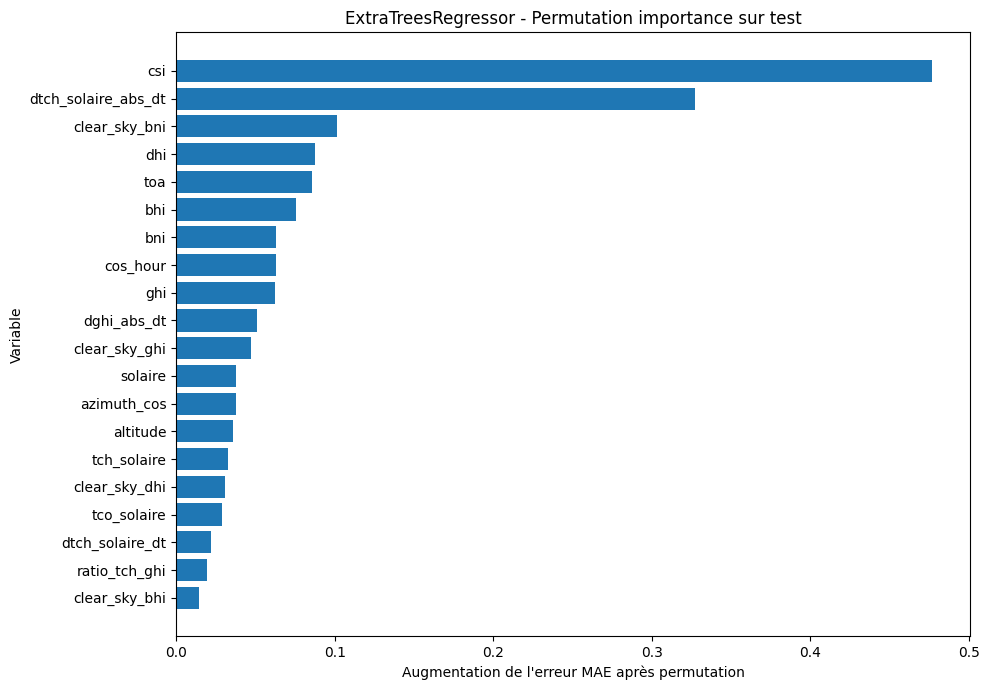
\includegraphics[width=0.8\textwidth]{img/var_imp.png}
    \caption{Permutation importance du modèle ExtraTrees sur l'ensemble de test.}
    \label{fig:var_imp}
\end{figure}

La permutation importance confirme les résultats précédents. Les variables \textit{csi} et \textit{dtch\_solaire\_abs\_dt} dominent clairement l'interprétation, avec des augmentations moyennes de MAE d'environ 0.37 et 0.32 après permutation.

La présence de \textit{clear\_sky\_bni} en troisième position est particulièrement importante. Elle montre que le modèle ne dépend pas uniquement des variations observées dans le passé, mais aussi du contexte physique de ciel clair et du potentiel de rayonnement direct. Autrement dit, le modèle apprend qu'une même perturbation atmosphérique n'a pas le même impact selon le niveau de rayonnement direct théoriquement disponible.

Les autres variables importantes, comme \textit{ghi}, \textit{bni}, \textit{dghi\_abs\_dt}, \textit{bhi}, \textit{clear\_sky\_ghi} et \textit{dhi}, confirment que les variations de production photovoltaïque sont fortement liées aux niveaux d'irradiance et aux changements rapides des conditions lumineuses. L'accord entre feature importance, SHAP et permutation importance renforce la confiance dans le modèle, car les variables dominantes ont un sens physique clair.


\chapter{Détection des événements extrêmes}

Au-delà de la performance moyenne en régression, il est utile d'évaluer la capacité du modèle à détecter les fortes variations de production, appelées ici rampes critiques. Cette analyse transforme temporairement le problème de régression en problème de détection binaire.

Un seuil Q90 est défini à partir de l'ensemble de développement. Les observations dont la variabilité est supérieure ou égale à ce seuil sont considérées comme critiques. Dans le notebook, le seuil obtenu est : $Q90 = 8.04$

La même logique est appliquée aux prédictions du modèle : si la variabilité prédite dépasse le seuil retenu, le modèle déclenche une alerte de rampe critique.

\section{Résultats avec le seuil Q90}


\begin{figure}[htbp]
    \centering
    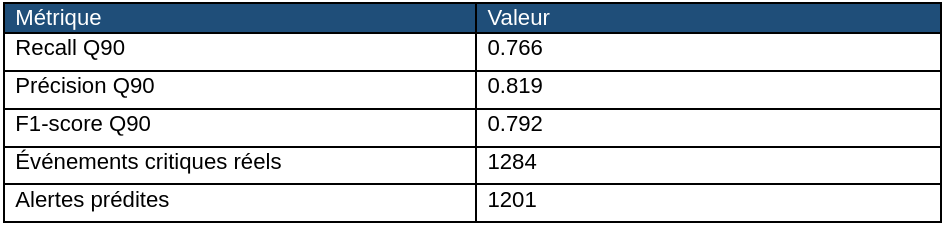
\includegraphics[width=0.9\textwidth]{img/tab_8_1.png}
    \caption{Résultats de détection des rampes critiques avec le seuil Q90.}
    \label{fig:tab_8_1}
\end{figure}

\begin{figure}[htbp]
    \centering
    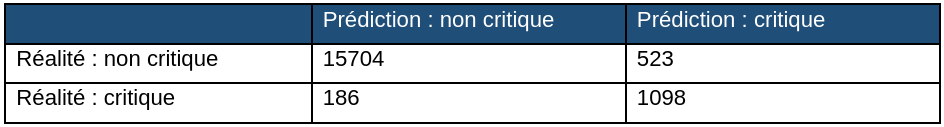
\includegraphics[width=0.9\textwidth]{img/tab_8_4.png}
    \caption{Matrice de confusion avec le seuil Q90.}
    \label{fig:tab_8_4}
\end{figure}


Avec le seuil Q90, le modèle détecte correctement 984 événements critiques parmi les 1284 réellement présents dans l'ensemble de test. Il manque donc 300 rampes critiques, soit environ 23.4 % des événements critiques.

En parallèle, le modèle produit 217 fausses alertes sur 16 227 situations non critiques. La précision atteint donc environ 81.9 \%, ce qui signifie que les alertes émises sont généralement fiables. Le recall de 76.6 % indique que le modèle identifie une grande partie des événements extrêmes, mais qu'une partie des rampes critiques reste non détectée.

Dans ce contexte, l'accuracy globale doit être interprétée avec prudence, car les événements critiques sont minoritaires. Les métriques les plus pertinentes sont donc le recall, la précision et le F1-score de la classe critique.

\section{Ajustement du seuil de décision}

Dans une application opérationnelle, le seuil utilisé pour définir les événements critiques réels peut être différent du seuil de décision appliqué aux prédictions. En abaissant le seuil de décision, le modèle devient plus sensible : il détecte davantage de rampes critiques, mais il génère aussi davantage de fausses alertes.

Le notebook teste plusieurs seuils et sélectionne un seuil permettant d'obtenir au moins 85 \% de recall tout en maximisant la précision. Le seuil optimisé obtenu est 7.372.

\begin{figure}[htbp]
    \centering
    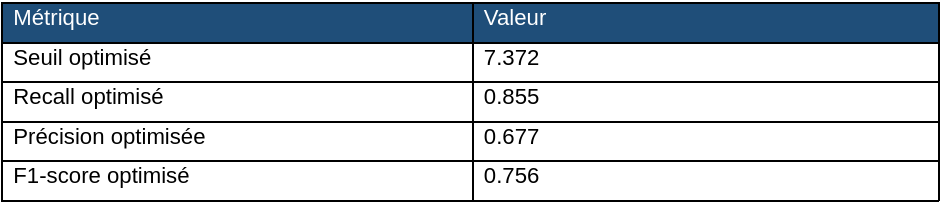
\includegraphics[width=0.9\textwidth]{img/tab_8_3.png}
    \caption{Résultats avec le seuil de décision optimisé.}
    \label{fig:tab_8_3}
\end{figure}

\begin{figure}[htbp]
    \centering
    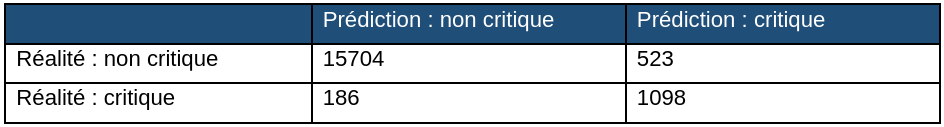
\includegraphics[width=0.9\textwidth]{img/tab_8_4.png}
    \caption{Matrice de confusion avec le seuil optimisé.}
    \label{fig:tab_8_4}
\end{figure}


Avec le seuil optimisé, le modèle détecte correctement 1098 événements critiques parmi les 1284 présents dans l'ensemble de test. Le recall atteint environ 85.5 \%, ce qui signifie que le modèle manque seulement 186 rampes critiques, soit environ 14.5 \% des événements critiques.

En contrepartie, le nombre de fausses alertes augmente de 217 à 523, et la précision diminue à environ 67.7 \%. Ce résultat traduit un compromis orienté vers une meilleure détection des événements extrêmes plutôt que vers une précision maximale des alertes.

Comparé au seuil Q90, le seuil optimisé améliore nettement la capacité de détection : le recall passe de 76.6 \% à 85.5 \%. Le choix final du seuil dépend donc du coût opérationnel relatif entre une rampe critique manquée et une fausse alerte.


\chapter{Conclusion générale}

Les parties finales du projet montrent une chaîne méthodologique complète allant de la construction des variables à l'interprétation du modèle final et à l'analyse opérationnelle des événements extrêmes.

Le modèle final retenu, ExtraTreesRegressor, conserve de bonnes performances sur l'ensemble de test, avec une MAE d'environ 0.467, un RMSE d'environ 0.986 et un R² d'environ 0.893. Ces résultats indiquent une bonne capacité de généralisation sur une période future indépendante.

L'interprétabilité confirme la cohérence physique du modèle. Les variables les plus importantes sont liées au CSI, à la variation récente de la production normalisée, aux variations de l'irradiance et au potentiel théorique d'irradiance directe sous ciel clair, en particulier \textit{clear\_sky\_bni}. Les analyses par feature importance, SHAP et permutation importance convergent donc vers la même conclusion : le modèle s'appuie principalement sur des signaux pertinents pour détecter les changements rapides de conditions solaires.

L'analyse des rampes critiques montre que le modèle ne se limite pas à de bonnes performances moyennes en régression. Avec le seuil Q90, les alertes sont plus fiables, avec une précision d'environ 81.9 \%. Avec le seuil optimisé, le modèle détecte davantage d'événements critiques, avec un recall d'environ 85.5 \%, au prix d'un plus grand nombre de fausses alertes.


\listoffigures

\end{document}
